\chapter{区分原初黑洞和天体物理黑洞}\label{chap:distinguish}

%We investigate how the next generation gravitational-wave (引力波) detectors, such as Einstein Telescope (ET) and Cosmic Explorer (CE), can be used to distinguish primordial black holes (原初黑洞) from astrophysical black holes (ABHs). Since a direct detection of sub-solar mass black holes can be taken as the smoking gun for 原初黑洞, we estimate the detectable limits of the abundance of sub-solar mass 原初黑洞 in cold dark matter by the targeted search for sub-solar mass 原初黑洞 binaries and binaries containing a sub-solar mass 原初黑洞 and a super-solar mass 原初黑洞, respectively. On the other hand, according to the different redshift evolutions of the merger rate for 原初黑洞 binaries and 天体物理黑洞 binaries, we forecast the detectable event rate distributions for the 原初黑洞 binaries and 天体物理黑洞 binaries by ET and CE respectively, which can serve as a method to distinguish super-solar mass 原初黑洞 from ABHs.

\section{背景介绍}
根据\lvc 科学组织最新发布的引力波瞬变目录2~\cite{Abbott:2020niy},目前一共探测到了50个致密双星并合事例。其中大多数都是双黑洞并合的事例。探测到了这么多双黑洞并合的引力波事件,加深了人类对宇宙的认识,但是还有很多问题需要回答。例如,这些双黑洞到底是如何形成和演化的,目前还是一个被广泛探讨的话题\cite{Bird:2016dcv,Sasaki:2016jop,Chen:2018czv,Clesse:2017bsw,Fishbach:2017dwv,Clesse:2016vqa,Antonini:2016gqe,Inayoshi:2017mrs,Ali-Haimoud:2017rtz,Perna:2019axr,Kavanagh:2018ggo,Rodriguez:2015oxa,Rodriguez:2016kxx,Park:2017zgj,Wu:2020drm,Belczynski:2014iua,Belczynski:2016obo,Woosley:2016nnw,Rodriguez:2018rmd,Choksi:2018jnq,2010AIPC.1314..291D,deMink:2016vkw}。

在引力波被探测到之前,由X射线观测到的黑洞的质量通常比较小\cite{Wiktorowicz:2013dua,Casares:2013tpa,Corral-Santana:2013uua,Corral-Santana:2015fud}。然而引力波观测到的双黑洞的质量要比X射线观测到的黑洞的质量要重很多。这一事实不禁让人们猜想观测到的双黑洞并合事件可能起源于恒星级质量的原初黑洞\cite{Bird:2016dcv,Sasaki:2016jop,Chen:2018czv,Clesse:2017bsw}。原初黑洞是在早期宇宙中由原初密度扰动的引力塌缩而形成的黑洞\cite{Hawking:1971ei,Carr:1974nx,Khlopov:2008qy,Sasaki:2018dmp}。其与起源于大质量恒星死亡而形成的天体物理黑洞经历了完全不同的演化历史。原初黑洞可能会构成部分的冷暗物质。而原初黑洞占冷暗物质的丰度,即$\fpbh$,已经受到了各种实验,例如星系外伽马射线\cite{Carr:2009jm}、伽马射线暴的femtolensing\cite{Barnacka:2012bm}、本星系中的白矮星\cite{Graham:2015apa}、Subaru/HSC微透镜\cite{Niikura:2017zjd}、开普勒毫-微透镜\cite{Griest:2013esa}、OGLE微透镜\cite{Niikura:2019kqi}、EROS/MACHO微透镜\cite{Tisserand:2006zx,Calcino:2018mwh}、超暗矮星系的动态加热\cite{Brandt:2016aco}、X射线/无线电\cite{Gaggero:2016dpq}、宇宙微波背景\cite{Ali-Haimoud:2016mbv,Blum:2016cjs,Horowitz:2016lib,Chen:2016pud,Poulin:2017bwe}以及引力波\cite{Wang:2016ana,Abbott:2018oah,Authors:2019qbw,Magee:2018opb,Wang:2019kaf,Chen:2019xse,Yuan:2019udt,Chen:2018rzo}等的限制。

除了原初黑洞模型,天体物理黑洞模型也可以解释\lvc 探测到的双黑洞。天体物理双黑洞的形成和并合是由演化环境主导的。在文献中,天体物理双黑洞模型主要有三种机制。第一种是\textit{动态形成}机制,即大质量恒星的演化形成黑洞,而黑洞被分离到星团核心,最后配对形成双黑洞系统\cite{Rodriguez:2015oxa,Rodriguez:2016kxx,Park:2017zgj}。第二种是\textit{经典孤立的双星演化}机制,即双黑洞是通过质量转移或公共包层抛射(common envelope ejection)而形成的\cite{Belczynski:2014iua,Belczynski:2016obo,Woosley:2016nnw,Rodriguez:2018rmd,Choksi:2018jnq}。第三种是\textit{化学均匀演化}机制,即由于氦气在整个包络体中的混合\cite{2010AIPC.1314..291D,deMink:2016vkw},使得恒星几乎在化学物质均匀的环境种演化形成黑洞。双黑洞的属性,如自旋\cite{Farr:2017uvj,Tiwari:2018qch,Ng:2018neg,Stevenson:2017dlk,Bogomazov:2018prw,Lopez:2018nkj,Sedda:2018nxm,Farr:2017gtv}、红移\cite{Fishbach:2018edt,Emami:2018taj,Bai:2018shq}和偏心率分布\cite{Samsing:2013kua,Samsing:2017xmd,Samsing:2017jnz,Lower:2018seu}等性质有可能区分不同机制的天体物理双黑洞模型。

在本节种,我们将探究通过使用引力波观测,特别是通过第三代地基引力波探测器,如爱因斯坦望远镜 (Einstein Telescope,简称ET)\cite{Punturo:2010zz}和宇宙勘探者(Cosmic Explorer,简称CE)\cite{Evans:2016mbw},来区分原初黑洞和天体物理黑洞的可能性。ET和CE有望每年探测到$\Od(10^5)$ \cite{Regimbau:2016ike,Vitale:2018yhm}个双黑洞并合事件,这个数目要远远大于比目前\lvc 探测到的双黑洞并合的数目。首先,我们考虑亚太阳质量($\lesssim 1\Msun$)的双黑洞。因为通常认为天体物理黑洞的质量要大于钱德勒赛卡质量极限($\sim 1.4 \Msun$)\cite{Chandrasekhar:1931ftj,Chandrasekhar:1931ih},所以直接探测到亚太阳质量的黑洞可以成为原初黑洞存在的关键证据。其次,我们考虑超太阳质量($\gtrsim 1\Msun$)的双黑洞。由于原初双黑洞和天体物理双黑洞的并合率随红移的演化可以有很大的不同,所以可探测双黑洞的事件数随红移的分布不同。我们分别估计ET和CE可探测到的原初黑洞和天体物理黑洞的事件数分布,这可以作为区分原初黑洞和天体物理黑洞的另一种方法。


%%%%%%%%%%%%%%%%%%%%%%%%%%%%%%%%%%%%%%%%%%%%%%%%%%%%%%%%%%%%%%%%%%%%%%%%%%%%%%%%
\section{\label{subsolar}通过亚太阳质量黑洞来区分原初黑洞和天体物理黑洞}
直接探测到亚太阳质量的黑洞可以作为原初黑洞的直接证据。可探测到的事件数不仅取决于原初双黑洞的并合率,而且还取决于引力波探测器的灵敏度。在下面的两个小节中,我们将分别考虑原初黑洞具有单色质量谱和一般质量谱的情况,来探讨不同的引力波探测器探测亚太阳质量黑洞的能力。

\subsection{\label{mono}原初黑洞具有单色质量谱的情况}
在本小节中,我们假设所有的原初黑洞都具有相同的质量,并通过对原初双黑洞的定向搜索(targeted search)来估计$\fpbh$的可探测极限。未探测到亚太阳质量双黑洞并合或相应的随机引力波背景,都可以对原初黑洞占冷暗物质的丰度$\fpbh$给出下限,即超过这个范围就有可能探测到原初黑洞。

\begin{figure}[h]
    \centering
    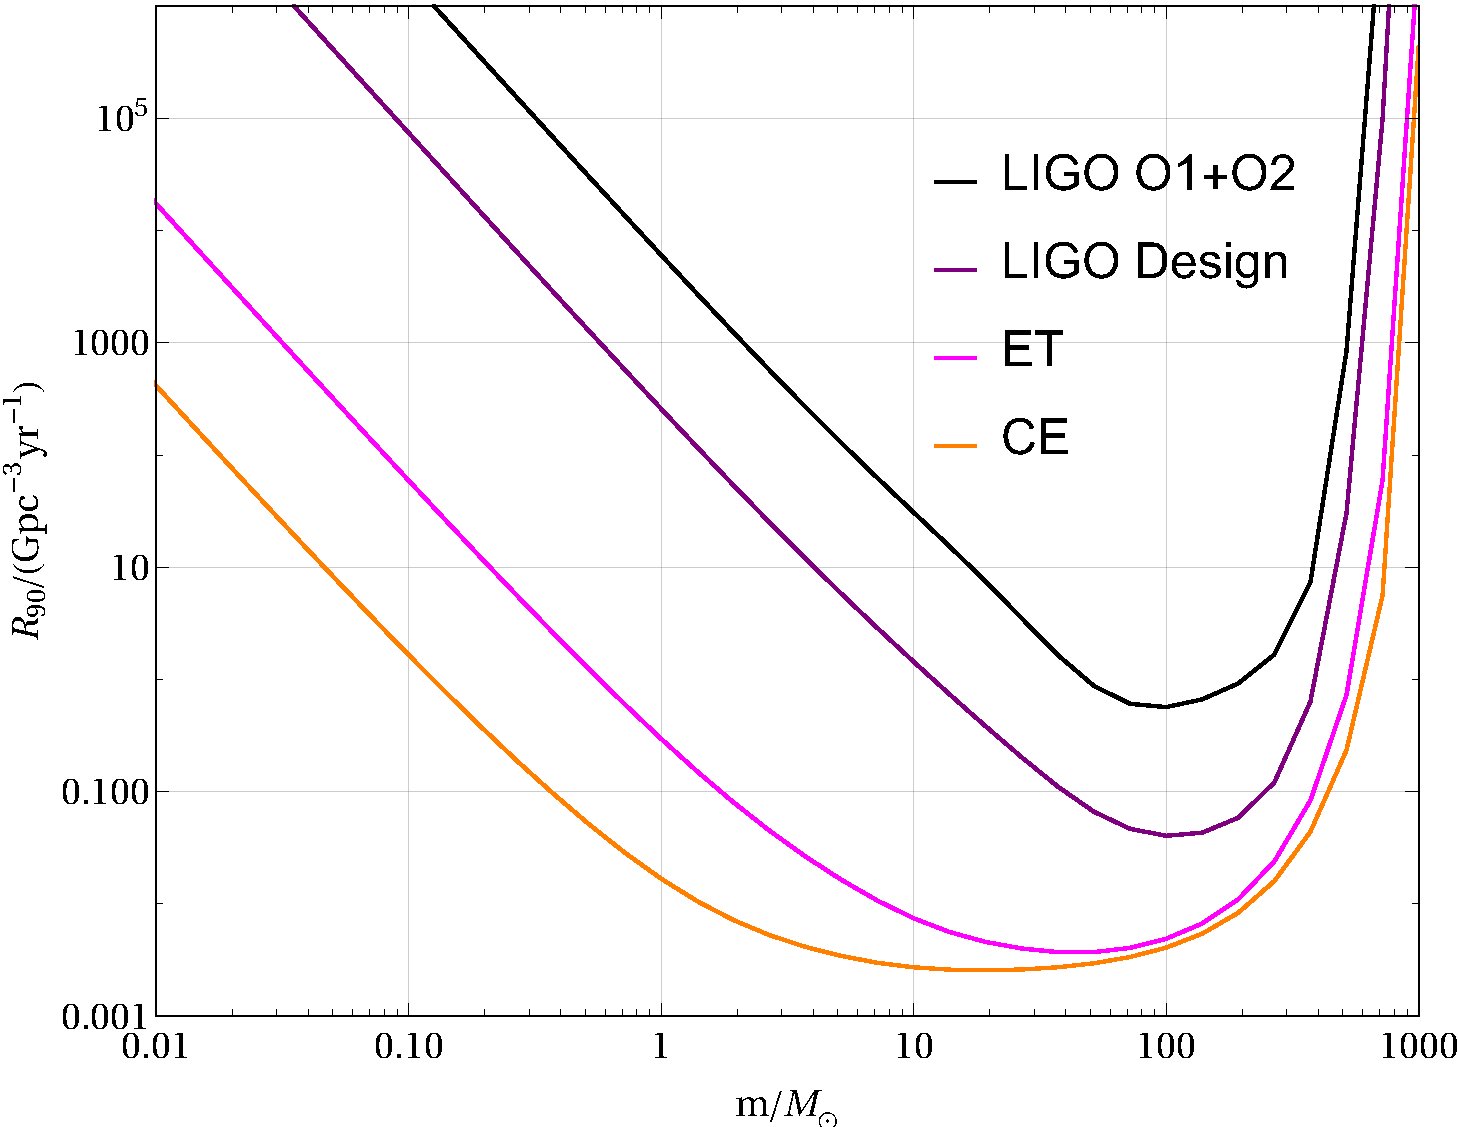
\includegraphics[width=0.9\textwidth]{R90.pdf}
    \bicaption{\label{R90_plot}LIGO O1 \& O2、LIGO设计、ET和CE给出的等质量双黑洞并合率的$90\%$上限$R_{90}$。}{The $90\%$ confidential upper limit on the binary merger rate, $R_{90}$, as a function of the masses of the equal-mass binary black holes for LIGO O1 \& O2, LIGO Design, ET and CE.}
\end{figure}

通过考虑所有原初黑洞和背景的线性密度涨落所提供的角动量,单色质量谱情况下的共动局部并合率$R(z)$随红移$z$的演化由以下公式给出\cite{Ali-Haimoud:2017rtz,Chen:2018czv}
\e\label{mono_R} 
R(z) = 3.9 \times 10^6 \times \({\frac{t(z)}{t_0}}\)^{-\frac{34}{37}}
m^{-32/37} f^2 \(f^2 + \seq^2\)^{-21/74},
\q 
其中,$m \Msun$是在源参考系测量的双黑洞的质量,而$\sigma_{\mathrm{eq}}$是在辐射-物质平衡时期,其余暗物质在$\Od(10^0\sim10^3) M_\odot$尺度上的密度扰动的方差。
参照文献\cite{Ali-Haimoud:2017rtz,Chen:2018czv},我们选择$\sigma_{\mathrm{eq}}\approx 0.005$。这里$\fpbh \equiv \Omega_{\mathrm{PBH}}/\Omega_{\mathrm{CDM}}$是冷暗物质中原初黑洞所占的能量密度的百分比,与非相对论物质中原初黑洞的总丰度$f$相关,具体关系为$\fpbh \approx f/0.85$。此外,$t(z)$是在红移$z$时的宇宙时间,而$t_0\equiv t(0)$是我们宇宙的年龄。

\begin{figure}[p!]
    \centering
    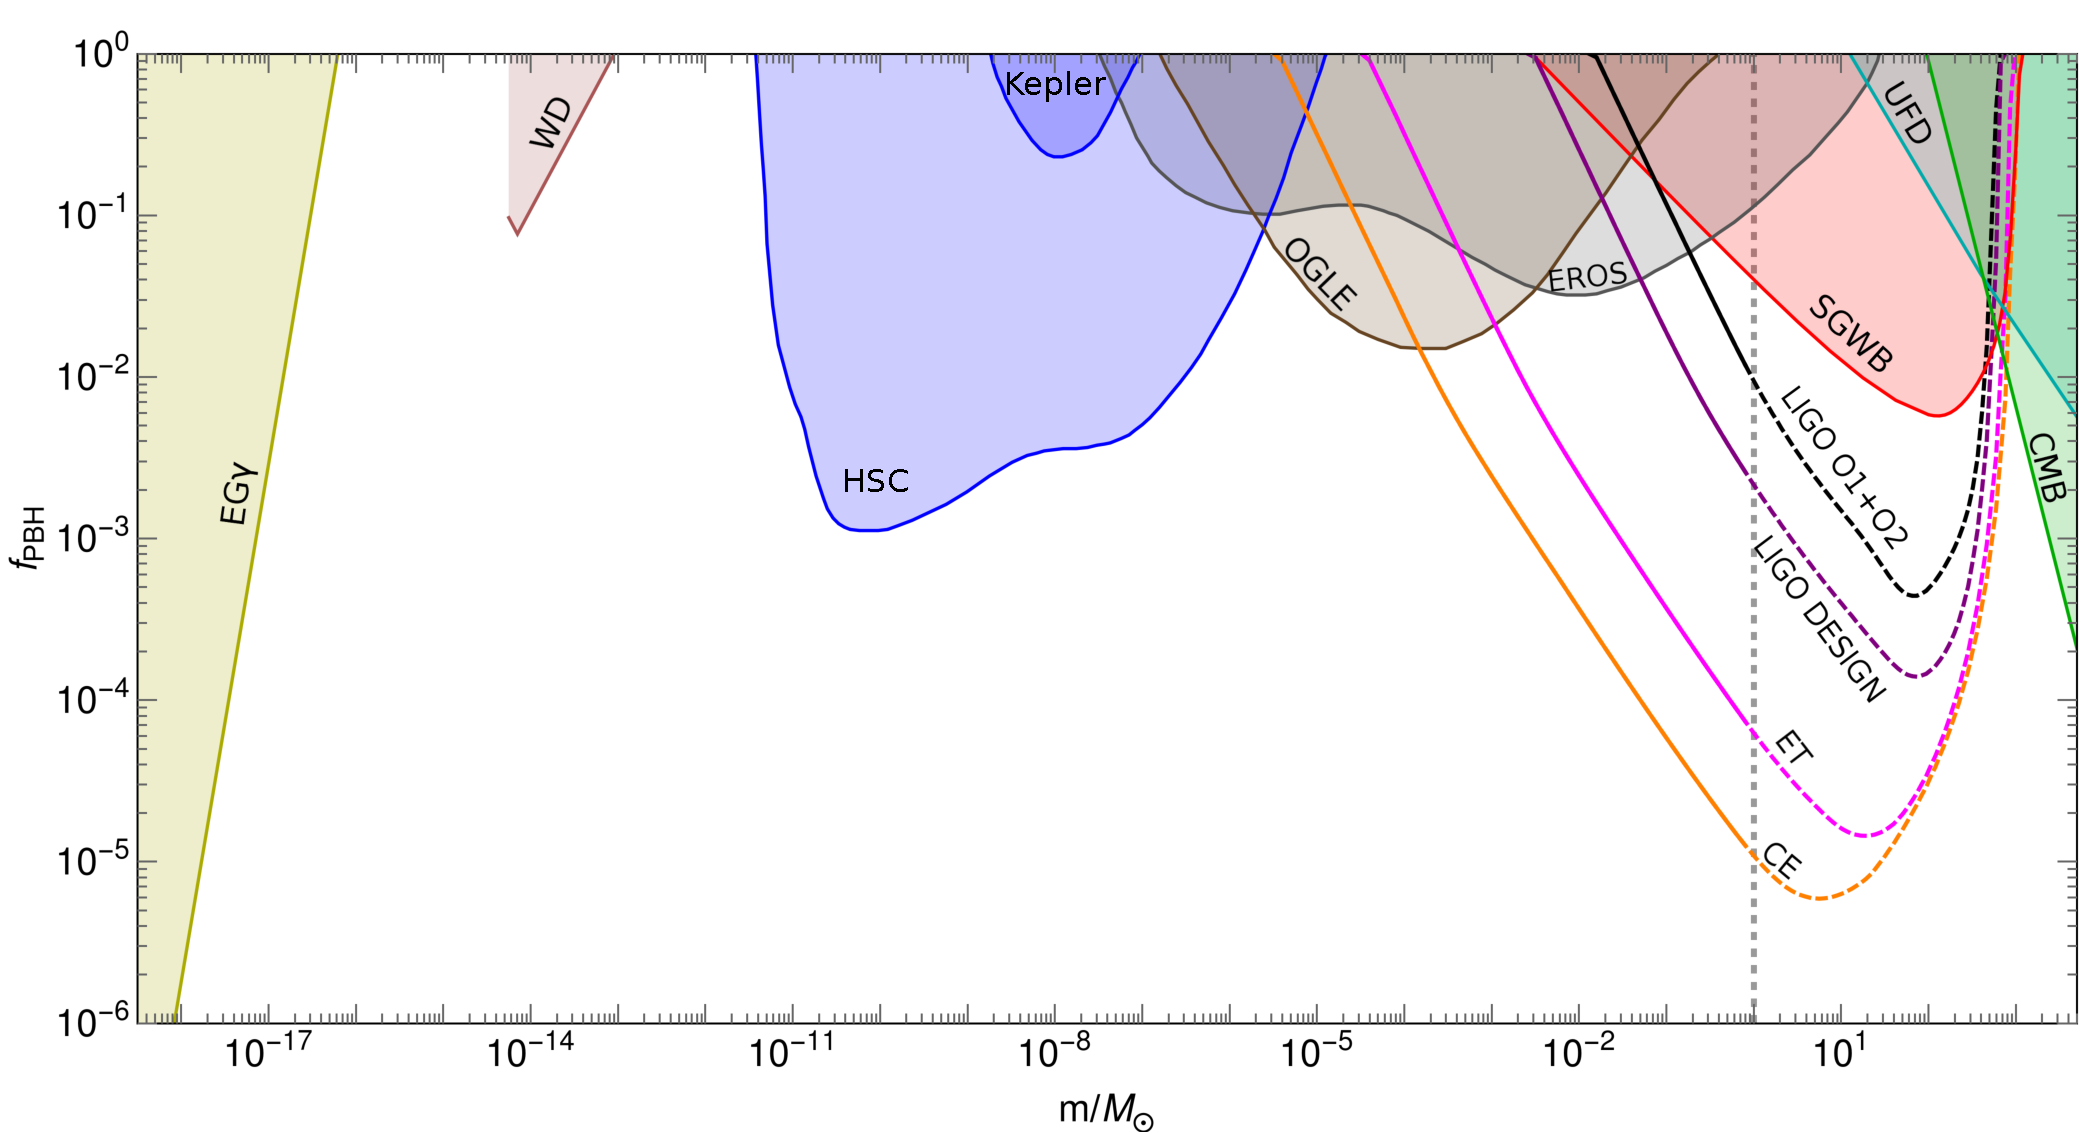
\includegraphics[width=\textwidth]{fpbh_m.pdf}
    \bicaption[由未探测到随机引力波背景和未探测到双黑洞并合对具有单质量分布的原初黑洞丰度$\fpbh$的限制。由于目前无法得知\lvc 探测到的双黑洞中到底有没有原初双黑洞,所以我们在图上$1\Msun$处用灰色竖线表示定向搜索的限制结果只对亚太阳质量的原初黑洞有效。黑色、紫色、洋红色和橙色曲线分别是LIGO O1/O2、LIGO设计、ET和CE的定向搜索给出的可探测极限。LIGO设计、ET和CE的观测时间均假设为$1$年。红色曲线代表由于LIGO O1和O2未探测到随机引力波背景给、本地星系中存在白矮星(WD) 、Subaru HSC微透镜(HSC)、开普勒毫/微透镜(Kepler)、EROS/MACHO微透镜(EROS)、OGLE微透镜(OGLE)、超暗矮星系(UFD)的动态加热以及微波背景辐射对$\fpbh$限制的结果。]{\label{fpbh1} 由未探测到随机引力波背景和未探测到双黑洞并合对具有单质量分布的原初黑洞丰度$\fpbh$的限制。由于目前无法得知\lvc 探测到的双黑洞中到底有没有原初双黑洞,所以我们在图上$1\Msun$处用灰色竖线表示定向搜索的限制结果只对亚太阳质量的原初黑洞有效。黑色、紫色、洋红色和橙色曲线分别是LIGO O1/O2、LIGO设计、ET和CE的定向搜索给出的可探测极限。LIGO设计、ET和CE的观测时间均假设为$1$年。红色曲线代表由于LIGO O1和O2未探测到随机引力波背景给出的$\fpbh$的上限。这里还给出了其他实验:星系外伽马射线(EG$\gamma$)\cite{Carr:2009jm}、本地星系中存在白矮星(WD) \cite{Graham:2015apa}、Subaru HSC微透镜(HSC)\cite{Niikura:2017zjd}、开普勒毫/微透镜(Kepler)\cite{Griest:2013esa}、EROS/MACHO微透镜(EROS) \cite{Tisserand:2006zx}、OGLE微透镜(OGLE)\cite{Niikura:2019kqi}、超暗矮星系(UFD)的动态加热\cite{Brandt:2016aco}以及微波背景辐射\cite{Ali-Haimoud:2016mbv,Blum:2016cjs,Horowitz:2016lib,Chen:2016pud,Poulin:2017bwe}对$\fpbh$限制的结果。
    }{Constraints on the abundance of primordial black holes, $\fpbh$, 
        with a monochromatic mass distribution both by the non-detection of SGWBs and the null targeted search result of binary black holes. The gray vertical line at $1\Msun$ indicates that the constraints from the targeted search are only valid for the sub-solar mass primordial black holes, because we yet cannot conclude that none of the ten binary black holes detected by \lvc\ are of primordial-origin binary black holes. The black, purple, magenta and orange curves are the results of targeted search from LIGO O1 \& O2, LIGO Design, ET and CE, respectively. The observing times of LIGO Design, ET and CE are all assumed to be $1$ year. The red curve is the updated upper bound of $\fpbh$ constrained by the non-detection of SGWB from both LIGO O1 and O2 searches. The results from other experiments are also shown here: extra-galactic gamma-ray (EG$\gamma$) \cite{Carr:2009jm}, existence of white dwarfs in our local galaxy (WD) \cite{Graham:2015apa}, Subaru HSC microlensing (HSC) \cite{Niikura:2017zjd}, Kepler milli/microlensing (Kepler) \cite{Griest:2013esa}, EROS/MACHO microlensing (EROS) \cite{Tisserand:2006zx}, OGLE microlensing (OGLE) \cite{Niikura:2019kqi}, dynamical heating of ultra-faint dwarf galaxies (UFD) \cite{Brandt:2016aco}, and accretion constraints by CMB \cite{Ali-Haimoud:2016mbv,Blum:2016cjs,Horowitz:2016lib,Chen:2016pud,Poulin:2017bwe}.}
\end{figure}

对某个引力波探测器,其预期可探测的事件数$\Nobs$为\cite{Chen:2018czv,Kavanagh:2018ggo}
\e\label{Nobs} 
\Nobs = \int R(z) \frac{\rd VT}{\rd z} \rd z,
\q 
其中$\rd VT/\rd z$是引力波探测器的可探测时空区域\cite{Abbott:2016nhf,Abbott:2016drs},表明该探测器对并合事件的选择效应。一般来说,$\rd VT/\rd z$是红移的函数,而且取决于双黑洞的属性$\xi$ (例如质量和自旋),其具体表达式为
\e 
\frac{\rd VT}{\rd z} = \frac{\rd V_c}{\rd z} \frac{\Tobs}{1+z} f(z|\xi),   
\q 
其中,$V_c$是共动体积,$\Tobs$是观测时间,分母$1+z$将宇宙时间从源参考系转换到探测器参考系。
这里$0 < f(z|\xi) < 1$是指在红移$z$时,在给定参数$\xi$下探测到双黑洞的概率\cite{OShaughnessy:2009szr}。
然后,可以通过使用最强事件统计范式(loudest event statistic formalism)来获得双黑洞并合率的$90\%$上限\cite{Biswas:2007ni}。
\e\label{R90} 
R_{90} = \frac{2.303}{VT},
\q
其中 
\e\label{VT}
VT = \int \frac{\rd VT}{\rd z} \rd z.
\q
我们采用了来自文献\cite{Abbott:2016nhf,Abbott:2016drs}的半解析近似的方法来计算$VT$。我们忽略了黑洞的自旋效应,并使用\texttt{IMRPhenomPv2}波形作为双黑洞并合的模板。此外,我们将单探测器的信噪比阈值设为$\SNR=8$作为可探测标准,这大致相当于两个探测器构成的探测网络的阀值为$12$。\Fig{R90_plot}显示了由\Eq{R90}估计出来的等质量双黑洞并合率的$90\%$上限。




\Fig{fpbh1}显示了LIGO O1/O2、LIGO设计、ET和CE通过定向搜索可得到的原初黑洞丰度$\fpbh$的可探测极限。我们假设在这些实验中没有探测到原初双黑洞。LIGO O1\& O2的总的有效观测时间为$165.6$天\cite{TheLIGOScientific:2016pea,TheLIGOScientific:2017qsa}。同时假定LIGO设计、ET和CE的运行时间都是全勤$1$年。文献\cite{Abbott:2018oah,Magee:2018opb}中通过对双黑洞的定向搜索,给出了质量范围为$\[0.2, 1\]\Msun$的亚太阳质量原初黑洞的$\fpbh$的上限。我们从几个方面来推广了文献\cite{Abbott:2018oah,Magee:2018opb}的结果。首先,我们采用了在文献\cite{Ali-Haimoud:2017rtz}中提出的并合率,与 文献\cite{Abbott:2018oah,Magee:2018opb}使用的来自文献\cite{Sasaki:2016jop}给出的并合率相比,我们所使用的并合率更全面地考虑了双黑洞系统的演化。其次,我们还通过提出用第三代引力波探测器(如CE和ET)来估计了$\fpbh$的可探测极限。最后,我们并不局限于$\[0.2, 1\]\Msun$的质量范围,而是扩展到探测器的可探测质量范围。在解释\Fig{fpbh1}的结果时应该小心。由于目前观测到的超太阳质量双黑洞是否属于原初双黑洞还有争议,我们用虚线来表明超太阳质量原初黑洞的可探测极限。
此外,当质量小于$0.2\Msun$,从引力波数据中搜索信号的难度会大幅增加。这是因为对于小质量系统,模板的起始频率也小;而做模板匹配所需的模板数量$\Ntemp$正比于最小质量$\Mmin$和起始频率$\fmin$\cite{Magee:2018opb}
\e 
\Ntemp \propto \(\Mmin  \fmin\)^{-8/3}.
\q
计算资源的急剧增加限制了目前的引力波探测能力,使其无法有效地处理质量远低于$0.2\Msun$的双黑洞系统。然而,在未来,这个问题可能会通过改进搜索算法或计算技术来解决。我们给出CE和ET的结果的主要目的是为了说明未来探测器的探测能力。还需要注意的是,文献\cite{Ali-Haimoud:2017rtz,Kavanagh:2018ggo}通过\lvc\ O1数据给出了质量范围为$[10, 300]\Msun$的原初黑洞的丰度$\fpbh$的上限。我们通过使用\lvc\ O1和O2数据更新了文献\cite{Ali-Haimoud:2017rtz,Kavanagh:2018ggo}的限制结果。所以我们得到的上限比文献\cite{Ali-Haimoud:2017rtz,Kavanagh:2018ggo}的结果更加严格。

由于\lvc 没有探测到随机引力波背景,文献\cite{Wang:2016ana}给出了$\fpbh$的上限。我们更新了\cite{Wang:2016ana}的结果,给出了$\fpbh$更严格的限制。通常人们可能会以为由定向搜索给出的原初黑洞丰度的限制要比由随机引力波背景给出的限制更严格。虽然来自轻质量的双黑洞并合产生的引力波信号非常微弱,无法被引力波探测器直接探测到,但是这些微弱的信号可以叠加形成一个可探测的随机引力波背景。所以未探测到随机引力波背景会对轻质量的原初黑洞的丰度给出更严格的限制。请看\Fig{fpbh1}中$0.1 \Msun$附近红曲线和黑曲线的交叉。其实,对于其他的探测实验(比如LIGO设计、ET和CE)也有类似的结果。

%%%%%%%%%%%%%%%%%%%%%%%%%%%%%%%%%%%%%%%%%%%%%%%%%%%%%%%%%%%%%%%%%%%%%%%%%%%%%%%%
\subsection{\label{general}原初黑洞具有一般质量谱的情况}

\lvc 在其O1和O2观测阶段的数据中搜索了两个黑洞都具有亚太阳质量的双黑洞系统,发现数据中并没有该类信号\cite{Abbott:2018oah,Magee:2018opb,Authors:2019qbw},并给亚太阳质量的原初黑洞的丰度给出了限制。然而,该搜索只考虑成分质量在$0.2\Msun$到$1\Msun$之间的原初双黑洞系统。在这一小节中,我们提出搜索两个质量分别是亚太阳质量和超太阳质量的黑洞构成的原初双黑洞系统。由于这样的系统可以发出更强的引力波,从而更容易被探测到。

在这里,我们将前一小节的讨论扩展到原初黑洞具有一般质量分布的情况。我们假设迄今为止由\lvc 观察到的所有双黑洞都是原初双黑洞。之前的工作\cite{Chen:2018rzo,Raidal:2017mfl,Kocsis:2017yty,Raidal:2018bbj} 通常选择一些特定的质量函数,例如幂律质量谱或对数正态质量谱,来描述原初黑洞质量分布。这些特定的质量谱通常来自特定的原初黑洞形成模型。在这里,我们采取一种与模型无关的方法,即将质量函数$P(m)$从$0.2 \Msun$到$100 \Msun$进行分段
\e\label{para} 
P(m) = \begin{cases} 
    P_0, & 0.2\, \Msun \leq m < 1\, \Msun \\
    P_1, & 1\, \Msun \leq m < 30\, \Msun \\
    P_2, & 30\, \Msun \leq m < 60\, \Msun \\
    P_3, & 60\, \Msun \leq m \leq 100\, \Msun
\end{cases}
\q 
其中$P_i = \{ P_0, P_1, P_2, P_3 \} $为四个常数,其满足归一化条件
\e 
\int P(m)\, \rd m = 0.8P_0 + 29P_1 + 30P_2 + 40P_3 = 1.
\q 
这里,四个$P_i$中只有三个是独立的,我们选择$\vth = \{P_1, P_2, P_3\}$作为自由参数。我们将用LIGO O1和O2探测到的10个双黑洞并合事件去拟合$\vth$。在本小节中,我们感兴趣的原初黑洞的质量范围为$\[\mmin, \mmax\] = \[0.2\Msun, 100\Msun\]$。这里$\mmin=0.2\Msun$对应于LIGO搜索亚太阳质量超轻双黑洞的质量下限\cite{Abbott:2018oah}。

在文献\cite{Chen:2018czv}中,我们给出了具有一般质量函数的原初双黑洞的并合率分布。对于一个归一化的质量谱,时间依赖的共动并合率密度$P(m|\vth)$为
\m\label{calR} 
\mR_{12}(t|\vth) &\app& 3.9 \cdot 10^6 \times \({\frac{t}{t_0}}\)^{-\frac{34}{37}} f^2 (f^2+\sigma_{\mathrm{eq}}^2)^{-{21\over 74}} \times (m_1 m_2)^{{3\over 37}} (m_1+m_2)^{36\over 37} \nonumber \\
&& \times  \min\(\frac{P(m_1|\vth)}{m_1}, \frac{P(m_2|\vth)}{m_2}\) \({P(m_1|\vth)\over m_1}+{P(m_2|\vth)\over m_2}\),
\n
其中双黑洞的分量质量$m_1$和$m_2$的单位为$\Msun$。通过对分量质量的积分,可以得到与时间(或红移)依赖的并合率为
\e\label{Rcal2}
\mR(t|\vth) = \int \mR_{12}(t|\vth)\ \rd m_1\, \rd m_2.
\q 
进而局域并合率密度为\cite{Chen:2018rzo}
\e 
\mR_{12}(t_0|\vth) = R\, p(m_1,m_2|\vth).
\q 
我们选取局域并合率$R \equiv \mR(t_0|\vth)$使得双黑洞并合的概率密度$p(m_1,m_2|\vth)$是归一的。

\begin{figure*}[htbp!]
	\centering
	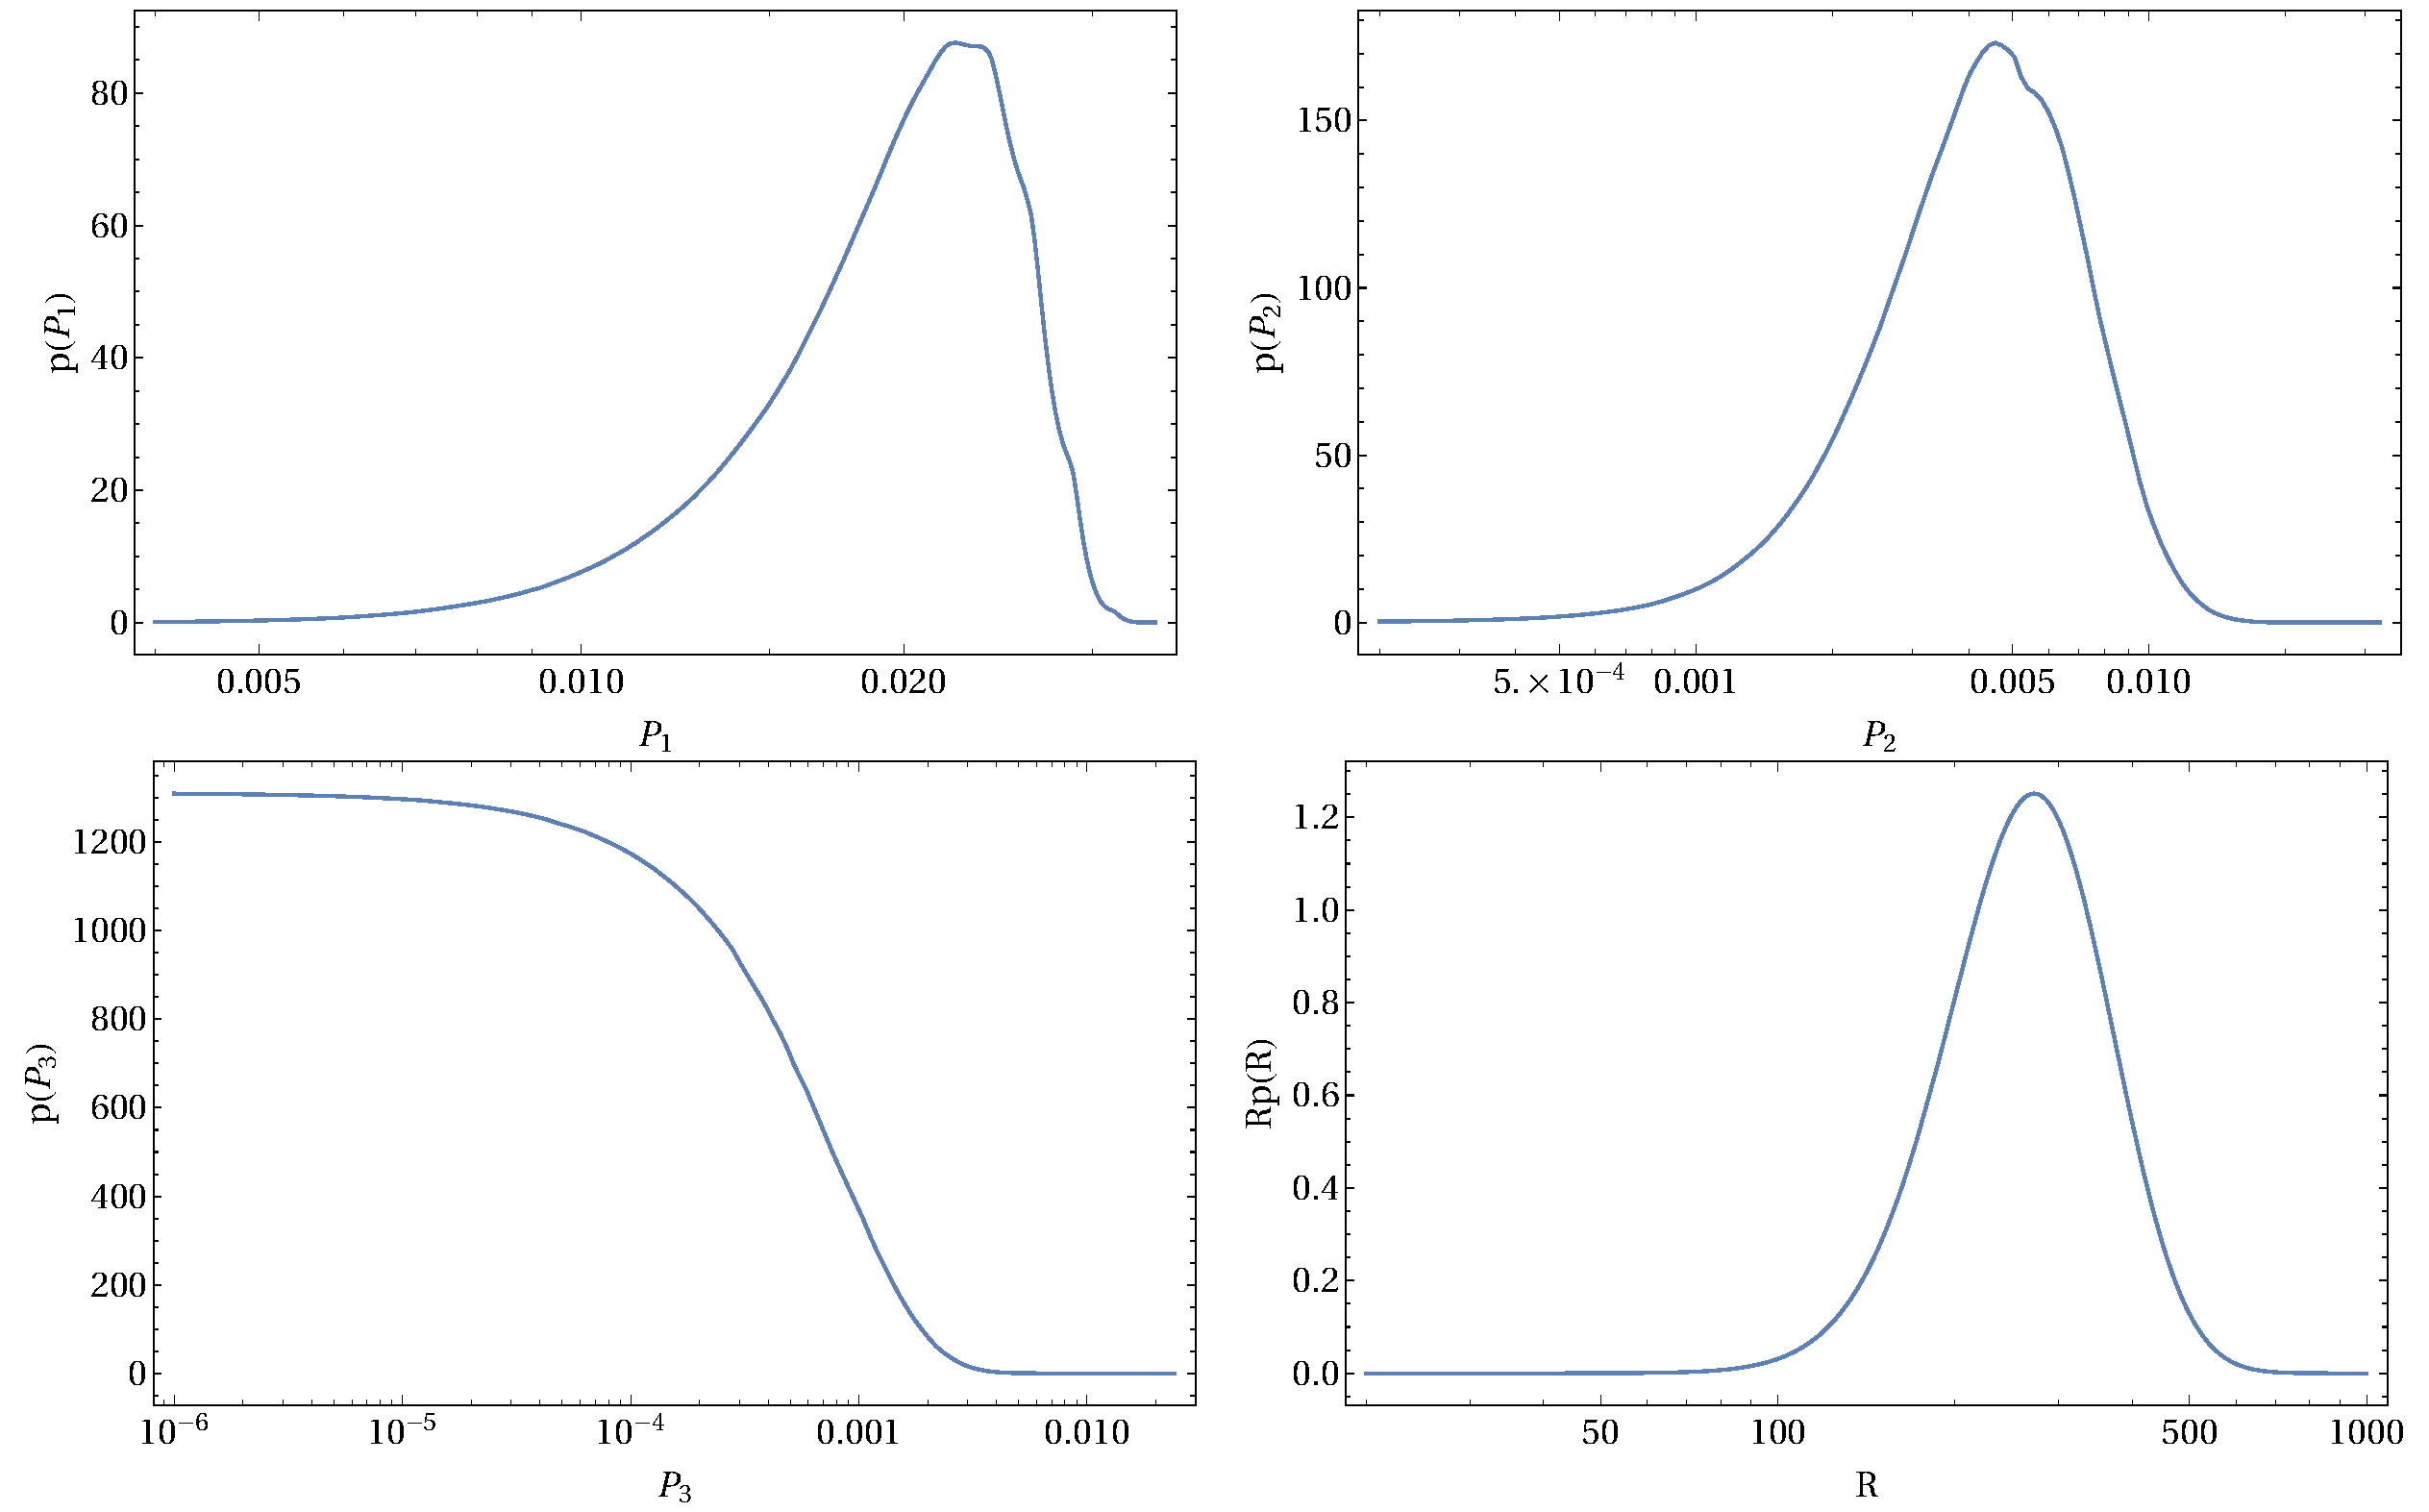
\includegraphics[width = \textwidth]{posts.pdf}
	\caption{\label{posts}
	$\{R, P_1, P_2, P_3\}$参数的后验分布。
	}{The posterior distributions for the free parameters $\{R, P_1, P_2, P_3\}$.}
\end{figure*}
为了从\lvc 观察到的并合事件中获取参数$\{\vth, R\}$的最佳拟合值,我们有必要从双黑洞质量分布做层次贝叶斯推断\cite{Abbott:2016nhf,Abbott:2016drs,TheLIGOScientific:2016pea,Wysocki:2018mpo,Fishbach:2018edt,Mandel:2018mve,Thrane:2018qnx}。
如果有$N$个双黑洞并合的数据,$\vd = (d_1, \dots, d_N)$,那么似然函数为\cite{Wysocki:2018mpo,Fishbach:2018edt,Mandel:2018mve,Thrane:2018qnx}
\e\label{likelihood}
p(\vd|\vth, R) \propto R^{N} e^{-R\, \beta(\vth)} \prod_i^N 
\int \rd\vla\ p(d_i|\vla)\ p(\vla|\vth),
\q 
其中$\vla \equiv \{m_1, m_2\}$。
由于在\lvc 做参数估计时,对于每个事件的质量参数选取的是平的分布,所以单个事件$p(d_i|\vla)$的似然函数与该事件的后验$p(\vla|d_i)$成正比。我们将使用\lvc 公开的10个双黑洞的后验分布\cite{TheLIGOScientific:2016pea,LIGOScientific:2018mvr}来估算\Eq{likelihood}的积分。同时,$\beta(\vth)$被定义为
\e 
\beta(\vth) \equiv \int \rd\vla\ VT(\vla)\ p(\vla|\vth),
\q 
其中$VT(\vla)$由\Eq{VT}给出。进而,我们可以直接估算后验概率分布$p(\vth, R|\vd)$为
\e\label{post} 
p(\vth, R|\vd) \propto p(\vd |\vth, R)\ p(\vth, R).
\q 
仿照\lvc \citep{Abbott:2016nhf,Abbott:2017vtc},我们选取$\vth$为平的分布,而$R$为对数平的分布,即
\e 
p(\vth, R) \propto \frac{1}{R}.
\q 
对\Eq{post}的 $R$进行积分,我们很容易得到边际化的后验分布 
\e\label{post_vth} 
p(\vth|\vd) \propto \[\beta(\vth)\]^{-N} 
\prod_i^N \int \rd\vla\ p(d_i|\vla)\ p(\vla|\vth).
\q
以上的后验分布已经被广泛运用于引力波参数推断中 \citep{Abbott:2016nhf,Abbott:2017vtc,TheLIGOScientific:2016pea,Abbott:2016drs,Fishbach:2017zga,Chen:2018rzo}。

\begin{figure}[h!]
    \centering
    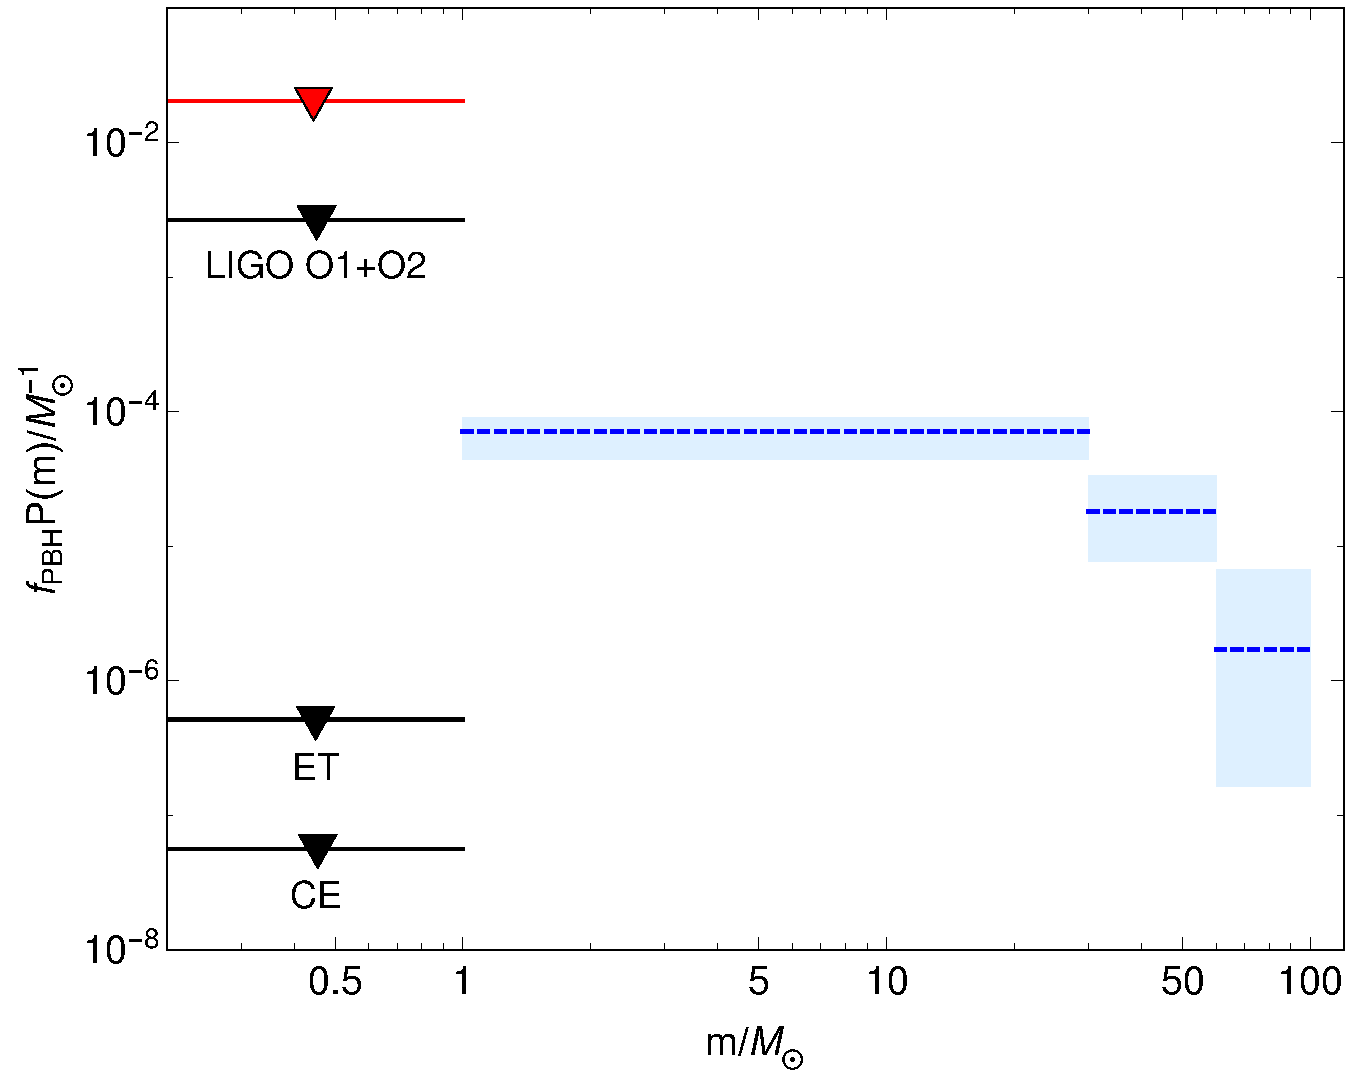
\includegraphics[width=\textwidth]{fpbhPmdm.pdf}
    \bicaption{\label{fpbhPmdm}
        对原初黑洞占冷暗物质丰度$\fpbh$的限制。蓝色区域是根据LIGO的O1和O2事件推断出来的对质量范围$1 \Msun \le m \le 100 \Msun$的限制。其中,中心虚线为中值,而阴影条代表$90\%$的泊松误差。在质量范围$[0.2, 1]\Msun$中显示的四条线分别代表了LIGO O1、LIGO O1 \& O2、ET和CE给出的限制。
    }{Constraints on the abundance of primordial black holes, $\fpbh$, in CDM.
    The blue regions with $1 \Msun \le m \le 100 \Msun$ 
    are inferred from LIGO's O1 and O2 events, 
    where the centered dashed lines are the median values and
    the shaded bars represent the $90\%$ Poisson errors.
    Four lines shown in the mass range $[0.2, 1]\Msun$ represent
    the constraints from null targeted searches of LIGO O1, 
    LIGO O1 \& O2, ET and CE, respectively.}
\end{figure}
\Fig{posts}给出了自由参数${R, P_1, P_2, P_3}$的后验分布。利用LIGO O1和O2探测到的10个双黑洞事件,我们得到参数$\{\vth, R\}$的中值和$90\%$的置信区间为
$P_1 = 2.1^{+0.7}_{-0.8} \times 10^{-2}$,
$P_2 = 5.4^{+4.7}_{-3.1} \times 10^{-3}$,
$P_3 = 5.1^{+15.2}_{-4.6} \times 10^{-4}$,
以及 $R = 308^{+193}_{-135}\, \gpcyr$。由此我们可以推断出原初黑洞占冷暗物质的丰度为$\fpbh = 3.3\,^{+2.3}_{-1.8} \times 10^{-3}$。
我们得到的原初黑洞的丰度与之前的估计是一致的,即$10^{-3} \lesssim \fpbh \lesssim 10^{-2}$。我们的结果证实了冷暗物质的主导部分不应该来源于质量范围为$[0.2, 100]\Msun$的原初黑洞\citep{Sasaki:2016jop,Ali-Haimoud:2017rtz,Raidal:2017mfl,Kocsis:2017yty,Chen:2018czv,Chen:2018rzo}。接下来我们将研究探测亚太阳质量双黑洞的可能性。
我们将质量范围为$[0.2, 1]\Msun$的原初黑洞的丰度记为 
\e 
\fpbhn \equiv \fpbh P_0 \,\Delta m_0,
\q
其中$\Delta m_0 = (1 - 0.2) \Msun = 0.8 \Msun$。
从上述得到的结果,我们可以通过LIGO的O1和O2数据直接推断出$\fpbhn$的上限为$\fpbhn \le 1.8 \times 10^{-3}$。未来,如果第三代地基引力波探测器投入运行,探测能力将大大增强。如果真的存在亚太阳质量双黑洞,我们将有更多机会探测到它们。除了寻找有两个亚太阳质量分量的双黑洞外,我们还建议寻找由一个亚太阳质量分量黑洞(质量在$[0.2, 1]\Msun$)和一个超太阳质量黑洞(质量在$[1, 100]\Msun$)构成的双黑洞系统。利用最强事件统计范式[见\Eq{R90}]和从LIGO的O1和O2数据推断出的$\vth$的值,$\fpbhn$可以被限制在一个前所未有的水平。假设没有双黑洞被探测到,ET可以得到$\fpbhn$的可探测极限为$\fpbhn \le 4.1 \times 10^{-7}$,而CE可以得到$\fpbhn$的可探测极限为 $\fpbhn \le 4.5 \times 10^{-8}$。\Fig{fpbhPmdm}显示了当原初黑洞具有一般的质量分布时,对$\fpbh$和$\fpbhn$的可探测限制。假设原初黑洞的质量在$[0.2, 1]\Msun$是平的分布,\Fig{fpbhPmdm}中的红线显示了未搜到亚太阳质量双黑洞而给出的$\fpbh$的上限。可以看出,搜索由亚太阳质量黑洞和超太阳质量黑洞构成的双黑洞得到的$\fpbh$的可探测极限,比搜索两个亚太阳质量的黑洞构成的双黑洞得到的$\fpbh$相比,将使$\fpbh$的可探测极限提高$\Od(10^2 \sim 10^3)$的数量级。


%%%%%%%%%%%%%%%%%%%%%%%%%%%%%%%%%%%%%%%%%%%%%%%%%%%%%%%%%%%%%%%%%%%%%%%%%%%%%%%%
\section{\label{stellar}用超太阳质量黑洞来区分原初黑洞和天体物理黑洞}



除了通过搜索亚太阳质量双黑洞外,还有一种方法是通过探索超太阳质量双黑洞的事件率的红移演化来区分原初黑洞和天体物理黑洞。在\cite{Chen:2018czv}中,我们发现原初双黑洞的并合率随着红移$z$的增加而增加,即$\mR(z) \propto t(z)^{-34/37}$,这与原初黑洞的丰度和质量函数都无关。然而,天体物理双黑洞预测的并合率首先会随着$z$的增加而增加,然后在某个小红移处达到峰值,最后会随着$z$的增加而迅速降低。\Fig{R_z}显示了原初双黑洞和天体物理双黑洞的并合率作为红移$z$的演化函数。可见这两个模型的并合率在红移越高时差异越大。目前,LIGO只能观测到低红移的双黑洞($z <1$),但未来的引力波探测器,如CE和ET,将能够探测到更高的红移($z \ge 10$)的双黑洞并合事件。
由于事件率随红移具有不同的分布,第三代地基探测器,如CE和ET,可以很好地区分原初黑洞和天体物理黑洞模型。 

\begin{figure}[h!]
    \centering
    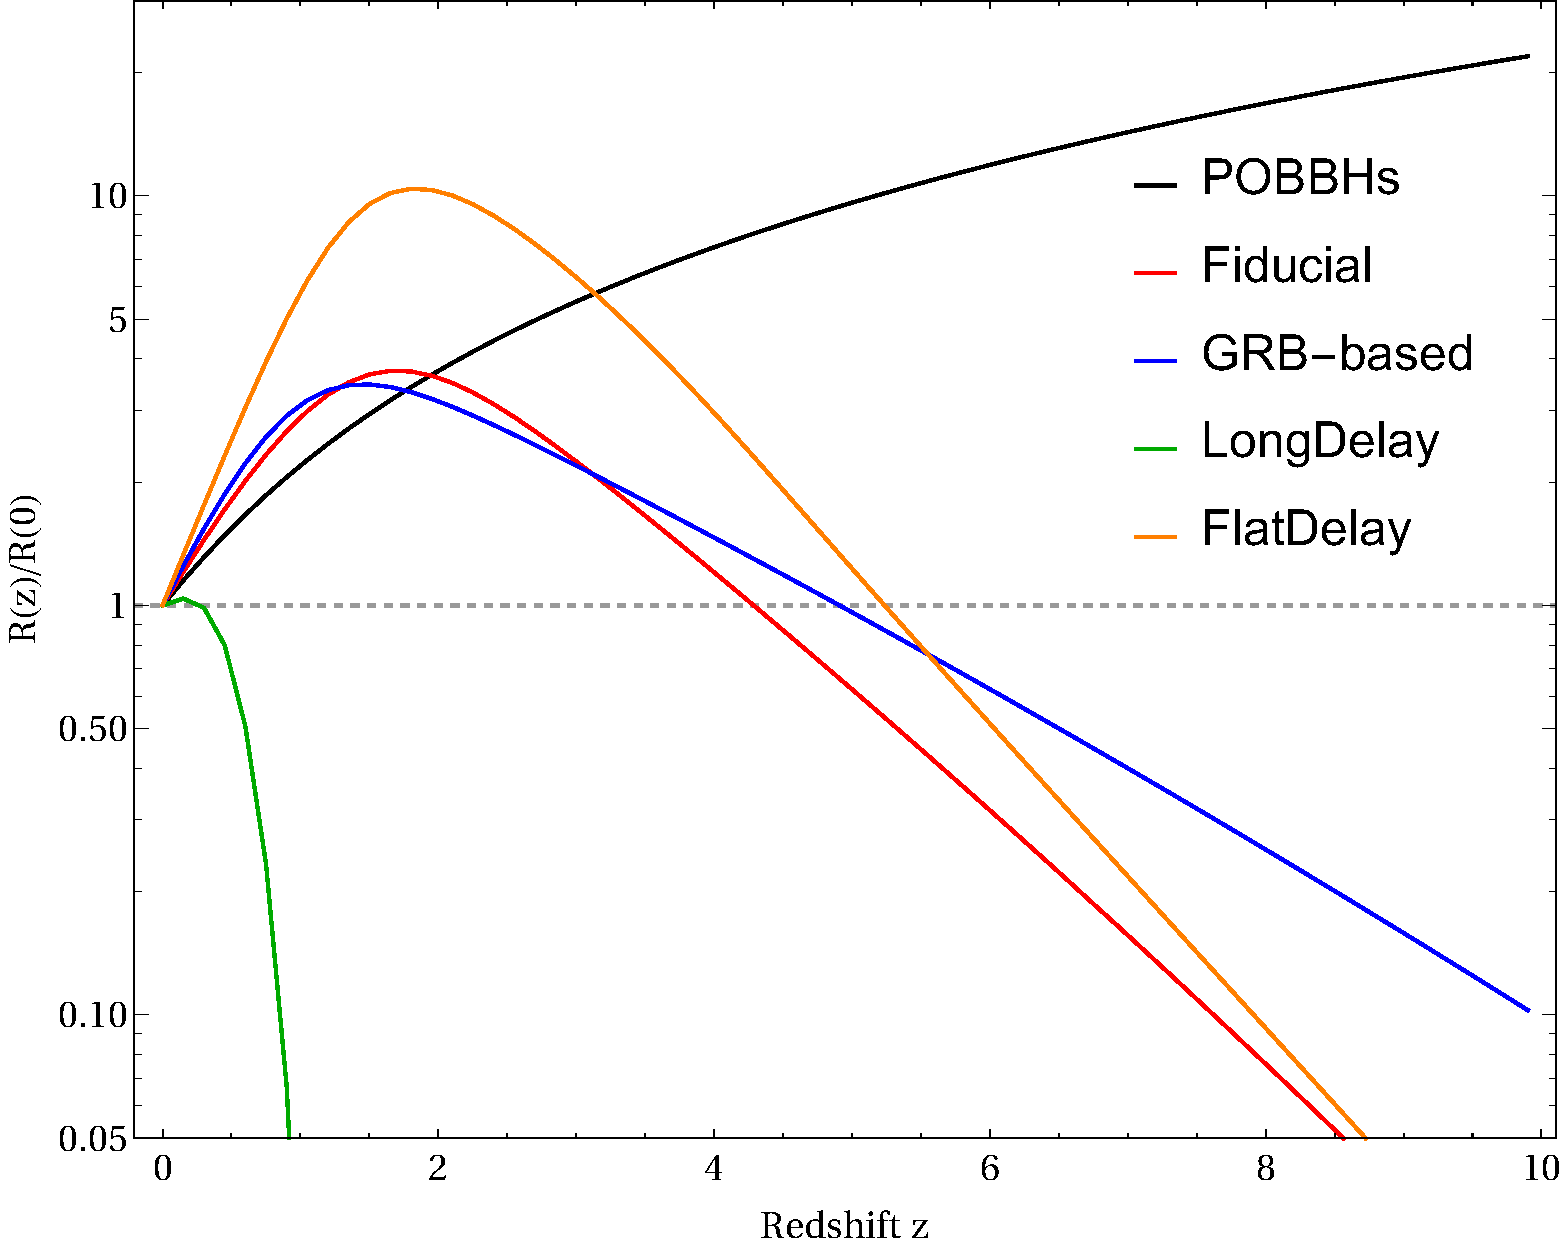
\includegraphics[width = 0.9\textwidth]{R_z.pdf}
    \bicaption{\label{R_z}
        原初双黑洞和天体物理双黑洞给出的归一化并合率的红移分布$R(z)/R(0)$。对于原初双黑洞和天体物理双黑洞,我们都只考虑双黑洞的质量范围为$5\Msun \leq m_2 \leq m_1 \leq 95 \Msun$。 我们假设原初黑洞具有一般的质量分布(见\Eq{para}),且用最佳拟合值来计算原初双黑洞的并合率。
    }{Redshift distribution of the normalized merger rate, $R(z)/R(0)$,
    for the primordial-origin binary black holes (POBBHs) and stellar-origin binary black holes, respectively.
    For both the primordial-origin binary black holes and stellar-origin binary black holes, we only count the binary black holes with masses 
    in the range of $5\Msun \leq m_2 \leq m_1 \leq 95 \Msun$.
    We assume primordial black holes have a broad mass distribution of Eq.~\eqref{para}, and the best-fits values are used to calculate the merger rate of primordial-origin binary black holes.}
\end{figure}

为了和之前的研究\citep{Abbott:2017vtc,Abbott:2017xzg}一致,
我们将双黑洞的分量质量限制在以下范围内 
$\mmin \leq m_2 \leq m_1$且$m_1 + m_2 \leq \mmax$。其中$ \mmin = 5\Msun$,$\mmax = 100\Msun$。
为了计算可观测事件率,我们首先需要知道并合率分布。
我们假设原初黑洞具有\Eq{para}的质量分布,并采用来自\ref{general}小节得到的最佳拟合值来计算并合率。而对于天体物理黑洞,并合率是天体物理黑洞的生成率$R_{\mathrm{birth}}(z,m)$与天体物理双黑洞的时间延迟分布$P_d(t_d)$的卷积\cite{Dvorkin:2016wac}
\e\label{sBHR}
\mR_{12}(z) = \int^{t_{\mathrm{max}}}_{t_{\text{min}}}  
R_{\mathrm{birth}}(t(z)-t_d, m_1) \times P_d (t_d)\ d t_d,
\q
其中$t_d$是时间延迟,$t(z)$双黑洞并合时的宇宙年龄。
生成率$R_{\mathrm{birth}}$可以通过以下方式估算出来 \citep{Dvorkin:2016wac}
\e\label{Rbirth}
R_{\mathrm{birth}}(t,m_{\mathrm{bh}})= \int \psi [t-\tau(m)]\, \phi(m)\, \delta(m- g_{\mathrm{bh}}^{-1}(m_{\mathrm{bh}}))\, dm,
\q
其中$m_{\mathrm{bh}}$是残余黑洞的质量,$\tau(m)$是质量为$m$的前身星的寿命,$\phi(m) \propto m^{-2.35}$是初始质量函数(IMF) \cite{Salpeter:1955it}。
我们考虑了``\textit{WWp}"的黑洞形成模型\citep{Woosley:1995ip},其中$m$和$m_{\mathrm{bh}}$存在以下关系
\e\label{mbhm}
\frac{m_{\mathrm{bh}}}{m}=A \left(\frac{m}{40\Msun} \right)^{\beta} \frac{1}{\left( \frac{Z(z)}{0.01 Z_\odot} \right)^{\gamma} +1},
\q 
其中$Z(z)$是金属丰度(具体形式见\cite{Belczynski:2016obo})。
\Eq{mbhm}中的参数值为:$A=0.3$,$\beta=0.8$和$\gamma=0.2$ \citep{Dvorkin:2016wac}。
解\Eq{mbhm}可以得到函数$m=g_{\mathrm{bh}}^{-1}(m_{\mathrm{bh}})$。
\Eq{Rbirth}中恒星形成率(SFR)$\psi(t)$可由以下公式计算 \citep{Nagamine:2003bd}
\e
\psi(z)= k \frac{a \exp[b(z-z_{m})]}{a-b+b \exp[a(z-z_{m})]},
\q
其中$z$是红移,$\{k, a, b, z_m\}$的参数值取决于具体的天体物理双黑洞的形成模型。在本节中,我们将考虑四个不同的天体物理双黑洞模型。

第一个为\texttt{Fiducial}模型,其中恒星形成率是对发光星系观测结果的拟合,拟合参数为$k=0.178 \, \Msun \, \mathrm{yr}^{-1}\, \mathrm{Mpc}^{-3}$, $z_{m}=2.00$, $a=2.37$, $b=1.80$ \cite{Vangioni:2014axa},时间延迟分布的形式为$P_{d} \propto t_{d}^{-1}$,并且$t_{\mathrm{min}} < t_{d} < t_{\mathrm{max}}$。其中最小延迟时间$t_{\mathrm{min}} = 50$\,Myr为双黑洞系统从形成直到并合的时间,最大延迟时间$t_{\mathrm{max}}$为哈勃时间\citep{TheLIGOScientific:2016wyq}。该模型对应于天体物理双黑洞模型的\textit{经典孤立双星演化}模型\cite{Dvorkin:2016wac}。

第二个是\texttt{GRB-based}模型,其中恒星形成率是利用高红移下的伽马射线暴(GRB)校准而得到的。这个模型中各参数取值为$k=0.146 \, \Msun \, \mathrm{yr}^{-1}\, \mathrm{Mpc}^{-3}$, $z_m=1.72$,$a=2.80$,$b=2.46$ \cite{Vangioni:2014axa}。

第三个是\texttt{LongDelay}模型,它与\texttt{Fiducial}模型基本相同,但假设最小时间延迟为$t_{\mathrm{min}}=5$Gyr,时间延迟明显变长。该模型可能与非常紧密的双星中快速旋转的大质量恒星的\textit{化学同质演化}模型相一致\cite{Mandel:2015qlu}。

最后一个是\texttt{FlatDelay} 模型,其假设时间延迟是平的分布,并且$t_{\mathrm{min}}=50$Myr和$t_{\mathrm{max}}=1$Gyr。
这个模型对应于\textit{动态形成}机制,即大多数的双星系统很可能发生在在宿主环境的极早期\cite{TheLIGOScientific:2016wyq}。

\begin{figure}[tbp!]
    \centering
    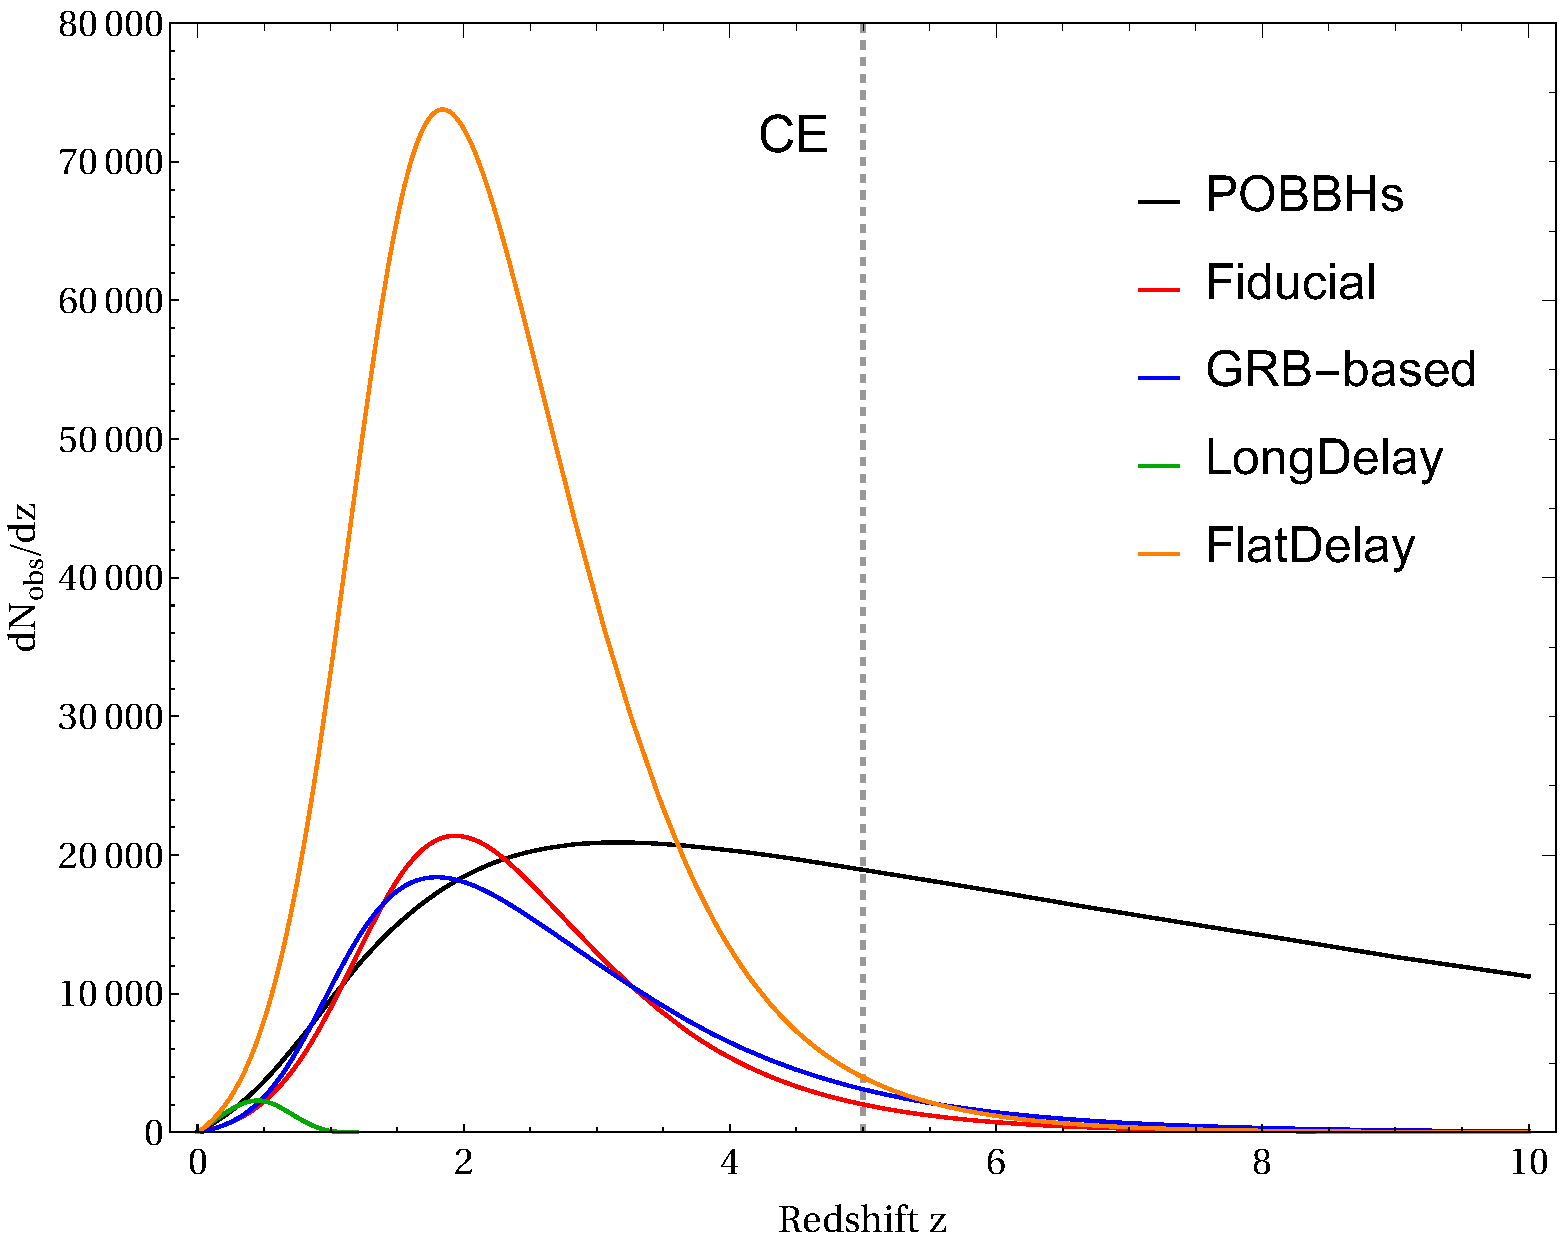
\includegraphics[width = 0.8\textwidth]{events_z_CE.pdf}\\
    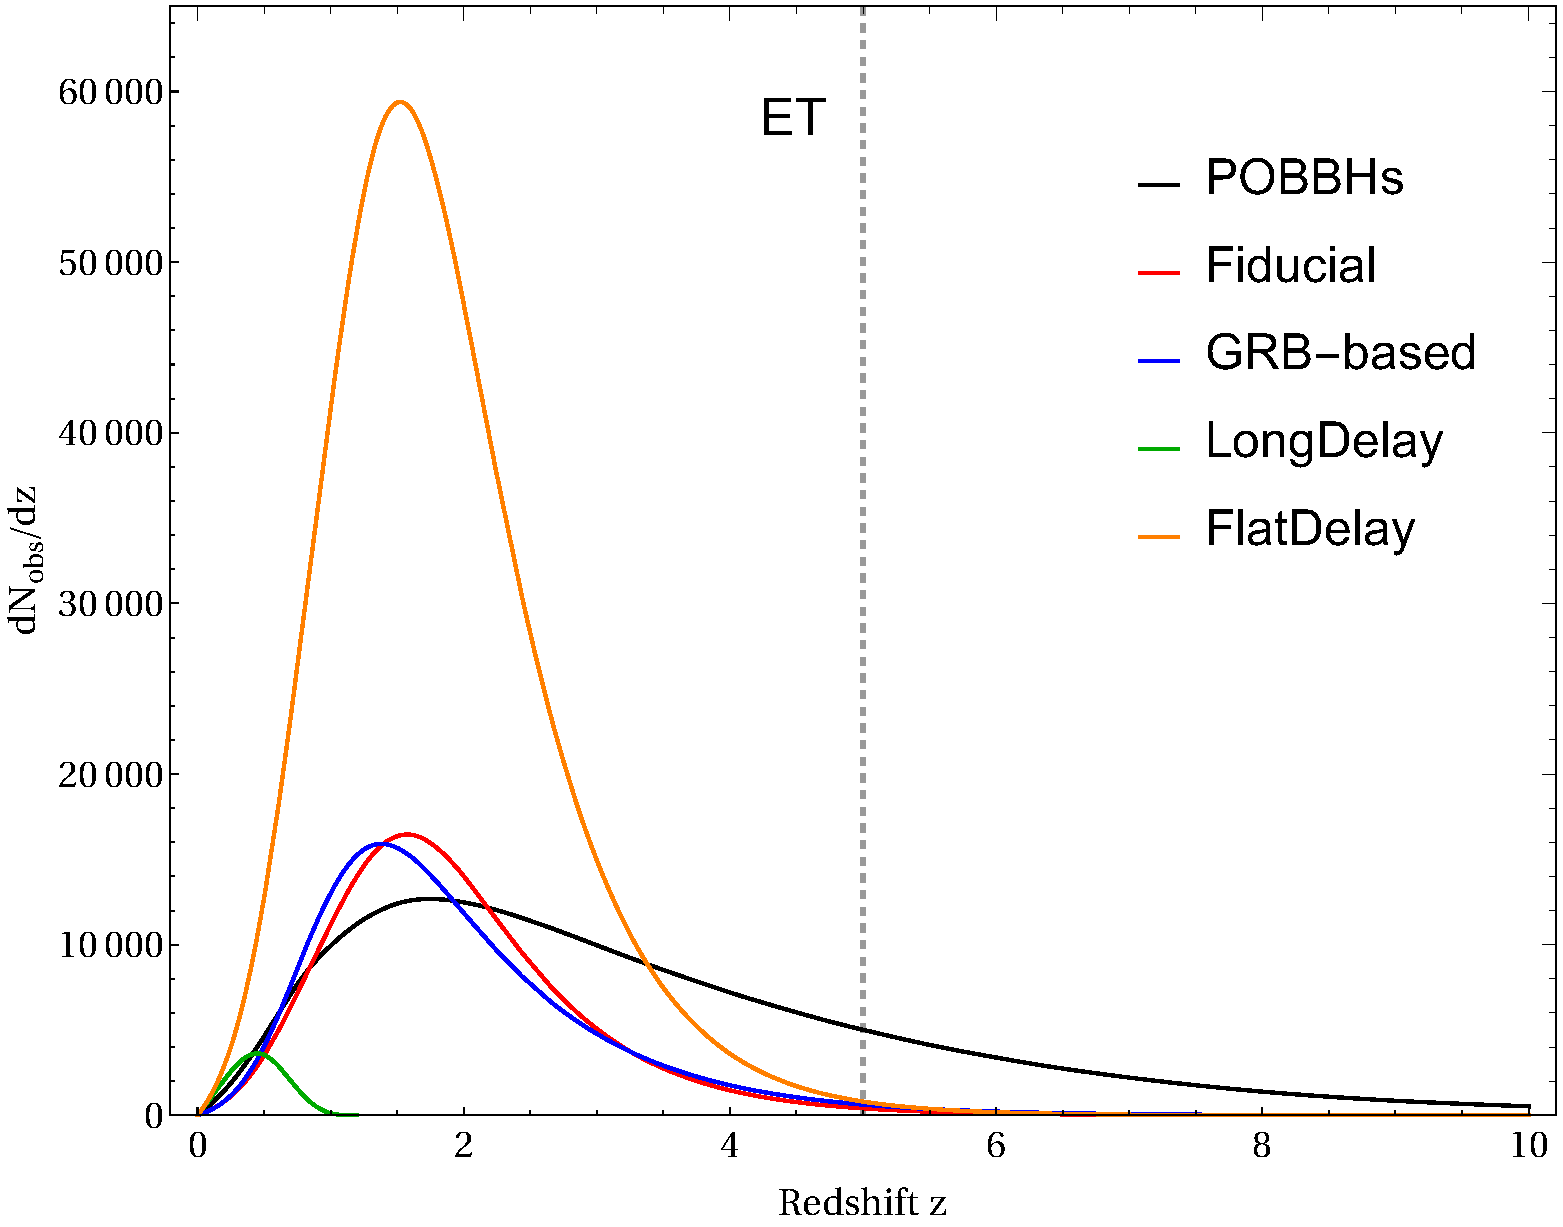
\includegraphics[width = 0.8\textwidth]{events_z_ET.pdf}
    \bicaption{\label{events_z}
        CE(上图)和ET(下图)对于双黑洞的可观测事件数密度$\rd \Nobs/\rd z$随红移的分布。对于原初双黑洞和天体物理双黑洞,我们都只考虑双黑洞的质量范围为$5\Msun \leq m_2 \leq m_1 \leq 95 \Msun$。 我们假设原初黑洞具有一般的质量分布(见\Eq{para})。
    }{Redshift distribution of the expected number density of observable binary black holes, $\rd \Nobs/\rd z$, for CE (top panel) and ET (bottom panel), respectively. For both the primordial-origin binary black holes (POBBHs) and stellar-origin binary black holes, we only count the binary black holes with masses in the range of $5\Msun \leq m_2 \leq m_1 \leq 95 \Msun$. We assume primordial black holes have a broad mass distribution of Eq.~\eqref{para}.}
\end{figure}

\begin{figure}[tbp!]
    \centering
    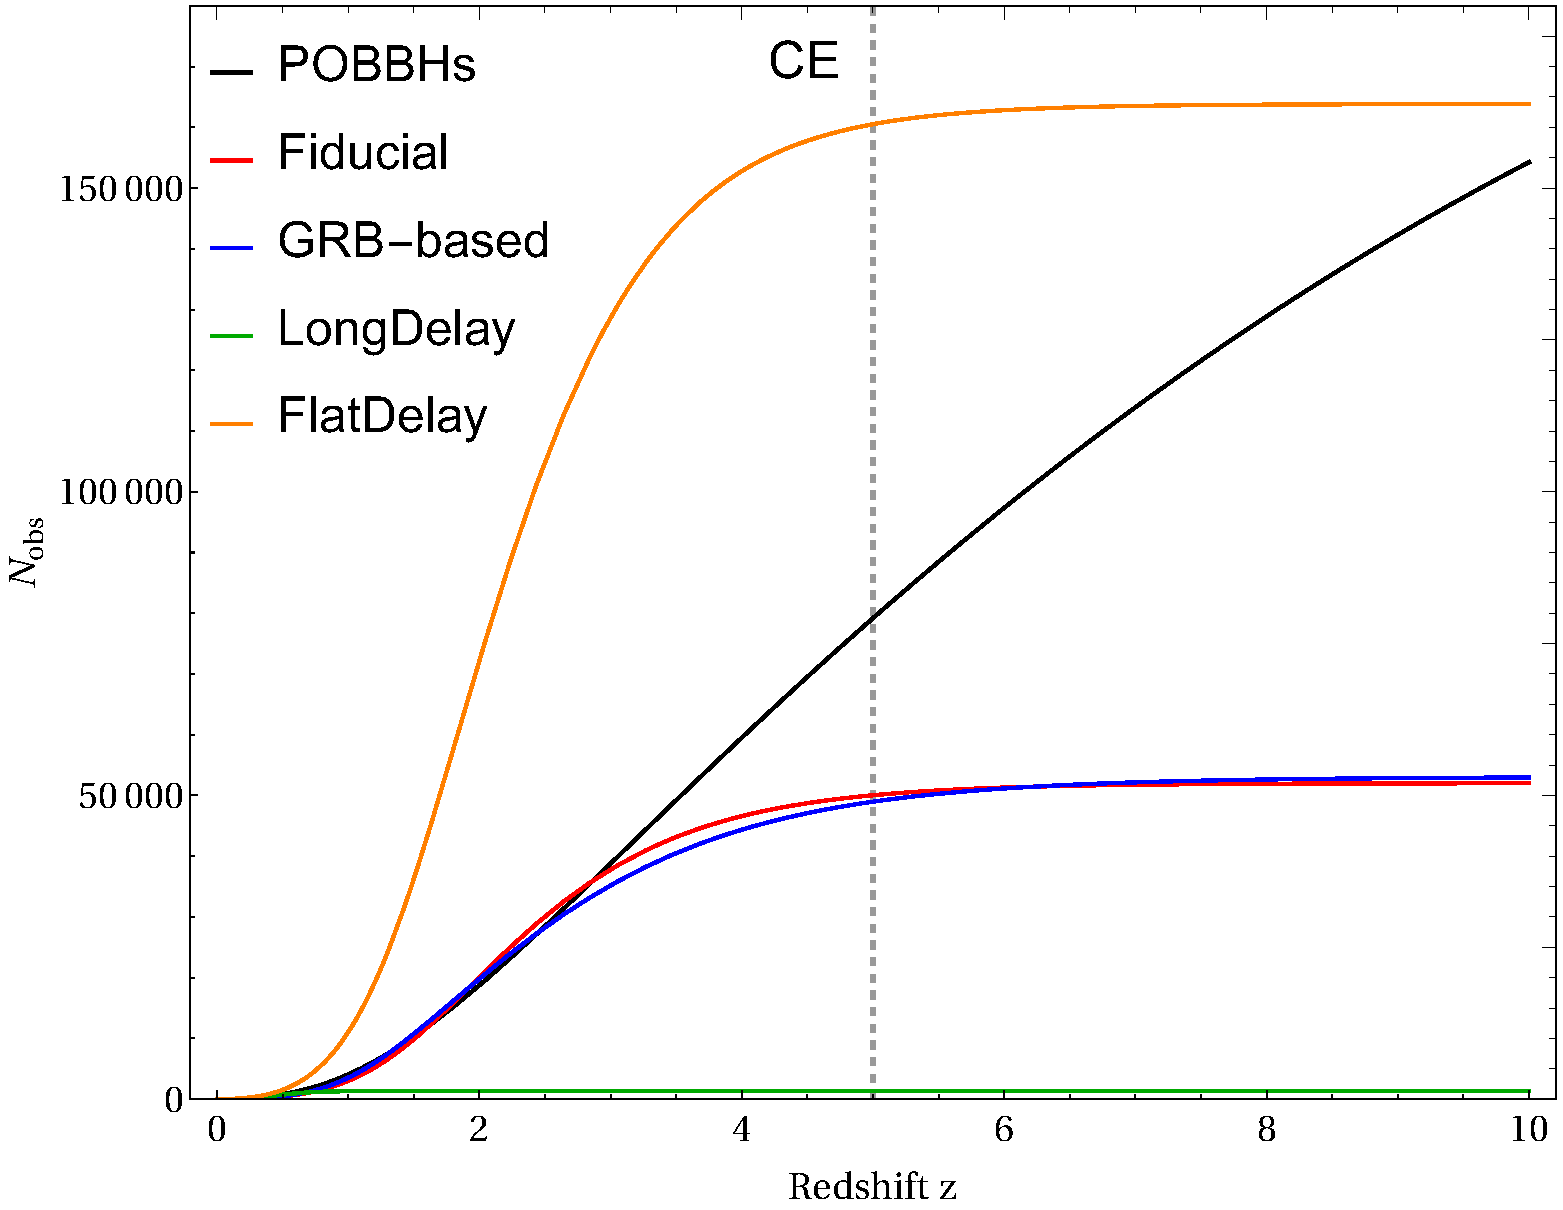
\includegraphics[width = 0.8\textwidth]{events_CE.pdf}\\
    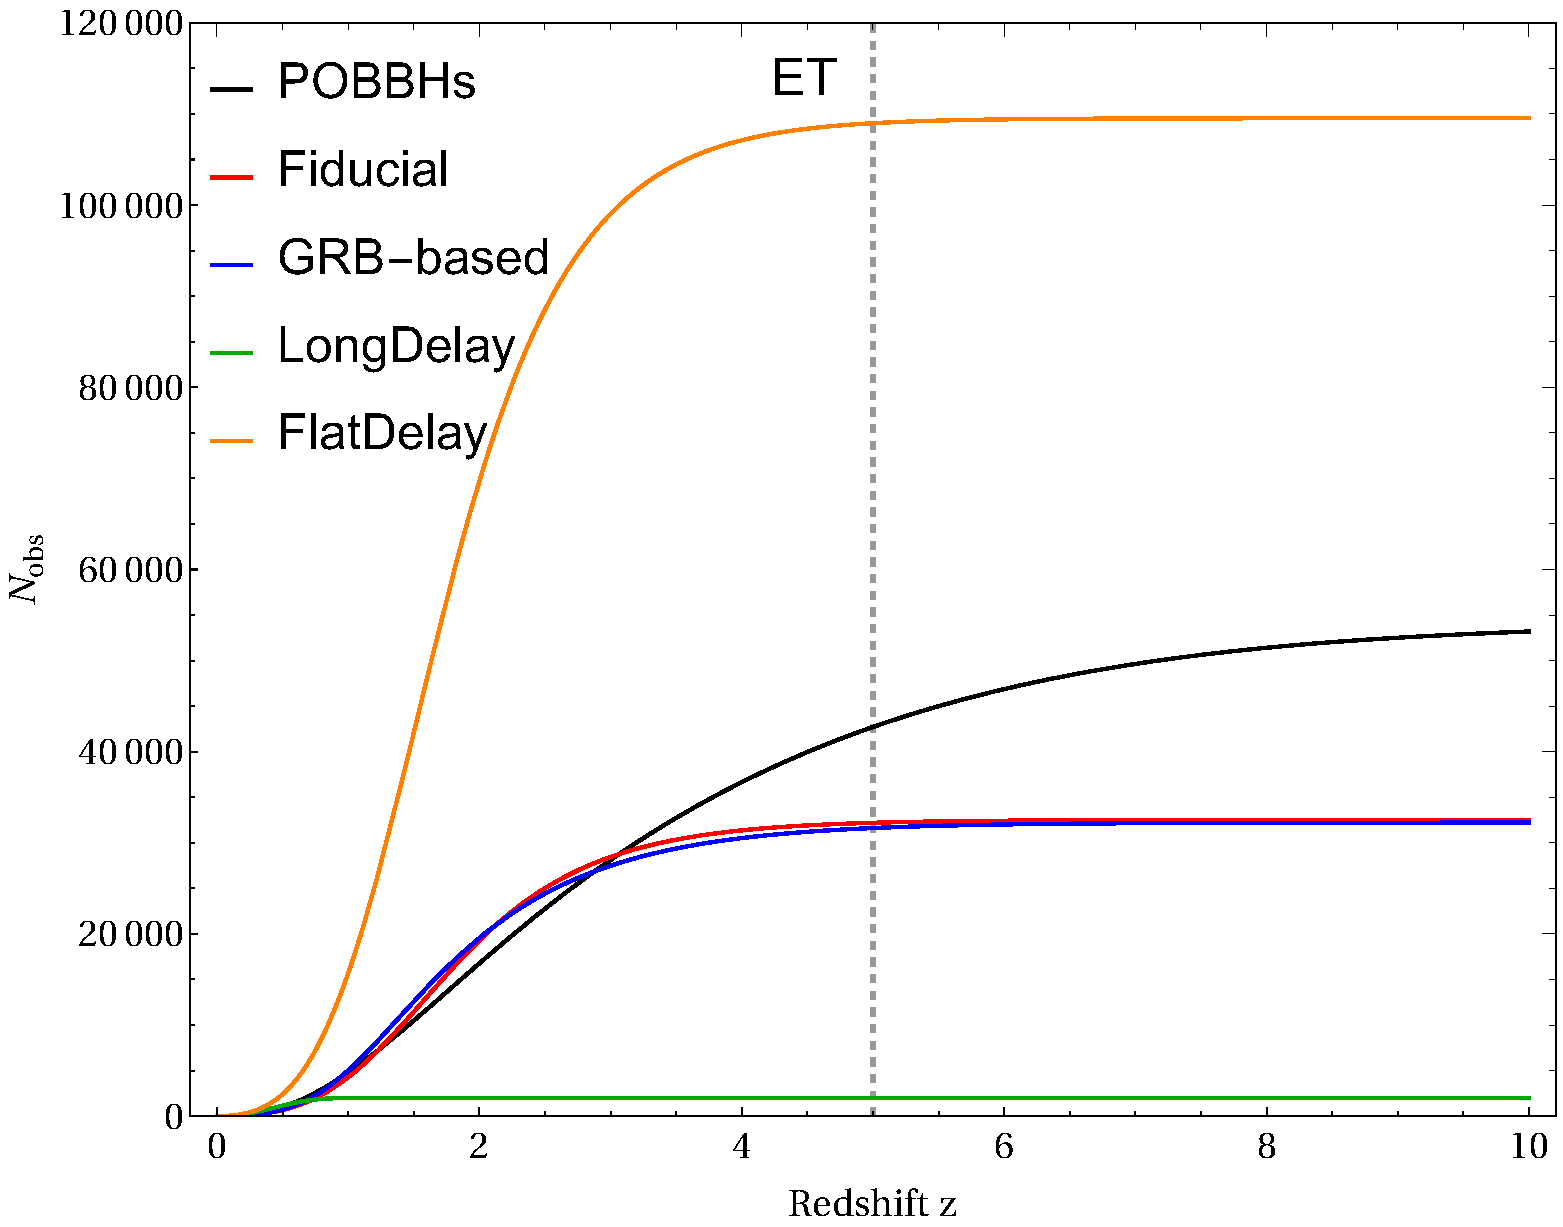
\includegraphics[width = 0.8\textwidth]{events_ET.pdf}
    \bicaption{\label{events}
        CE(上图)和ET(下图)对双黑洞的可观测总数$\Nobs$随红移的分布。对于原初双黑洞和天体物理双黑洞,我们都只考虑双黑洞的质量范围为$5\Msun \leq m_2 \leq m_1 \leq 95 \Msun$。 我们假设原初黑洞具有一般的质量分布(见\Eq{para})。
    }{Redshift distribution of the total number of observable binary black holes,
        $\Nobs$, for CE (top panel) and ET (bottom panel), respectively.
        For both the primordial-origin binary black holes (POBBHs) and stellar-origin binary black holes, we only count the binary black holes with masses 
        in the range of $5\Msun \leq m_2 \leq m_1 \leq 95 \Msun$.
        We assume primordial black holes have a broad mass distribution of Eq.~\eqref{para}.}
\end{figure}

\Fig{R_z}比较了原初双黑洞模型和不同天体物理双黑洞模型的归一化并合率$R(z)/R(0)$的红移分布。由图可知,随着红移的增加,\texttt{LongDelay}模型的并合率迅速下降;而与\texttt{Fiducial}和\texttt{FlatDelay}模型相比,\texttt{GRB-based}模型在高红移时的并合率相对较高。此外,所有天体物理双黑洞模型的并合率在高红移时都有所下降,而原初双黑洞模型的并合率在高红移时有所上升。
对于某个引力波探测器,与红移依赖的可观测事件数密度可以用以下公式计算出来
\e\label{event_density} 
\frac{\rd \Nobs}{\rd z} = \int \rd m_1 \rd m_2\, \mR_{12}(z)\,
\frac{\rd VT}{\rd z}.
\q 
对红移$z$进行积分,可得出可观测事件的总数$\Nobs$,
\e\label{Nobs2} 
\Nobs = \int \rd z \frac{\rd \Nobs}{\rd z}.
\q 
需要注意的是当$m_1 = m_2 = m$时,\Eq{Nobs}是\Eq{Nobs2}的一个特例。
\Fig{events_z}显示了CE和ET对双黑洞的可观测数密度随红移的分布$\rd \Nobs/\rd z$。
\Fig{events} 显示了CE和ET的对双黑洞的可观测总数$\Nobs$随红移的分布。
像CE和ET这样的第三代引力波探测器预计每年会探测到$\Od(10^5)$个双黑洞并合事件,并且可探测更高的红移。因为原初双黑洞和天体物理双黑洞的$\rd \Nobs/\rd z$随红移分布有很大的不同,所以可用来区分这两种双黑洞形成模型。特别是,对于我们所讨论的所有$4$种天体物理双黑洞模型来说,高红移($z>5$)对可观测数密度的贡献可以忽略不计,因此可观测事件的总数$\Nobs$在$z>5$时接近于一个常数。然而,对于原初双黑洞来说,高红移的贡献不能被忽略,因此当$z>5$时,$\Nobs$仍然会增加。



%%%%%%%%%%%%%%%%%%%%%%%%%%%%%%%%%%%%%%%%%%%%%%%%%%%%%%%%%%%%%%%%%%%%%%%%%%%%%%%%
\section{\label{discuss}总结和讨论}

\lvc 已经探测到几十个双黑洞并合产生的引力波事件,为人类探索宇宙打开了另一扇窗口。理解这些双黑洞是如何形成及演化的,是一个有待解决的科学问题。在本章中,我们探讨了通过下一代地基引力波探测器,比如ET和CE,来区分原初黑洞和天体物理黑洞的可能性。

我们首先研究了直接探测亚太阳质量双黑洞并合的可能性。如果搜索到亚太阳质量的双黑洞并合,那将是原初黑洞存在的强有力证据。对于具有单色质量谱的原初黑洞模型,我们估计和预测LIGO、ET和CE对原初黑洞占冷暗物质丰度$\fpbh$的可探测限制。只有$\fpbh$大于某个限制,才有可能被相应的探测器探测到。相应的结果见\Fig{fpbh1}。为了得到更好的限制,我们进一步考虑了去搜索由一个亚太阳质量黑洞和另一个超太阳质量黑洞构成的双黑洞系统。由于质量更大,所以这样的双黑洞比两个黑洞的质量都是亚太阳质量的双黑洞更容易被探测到。我们预测,如果ET和CE没能探测到这样的双黑洞系统,那么质量为$[0.2, 1]\Msun$的原初黑洞占冷暗物质的丰度会被限制到$\Od(10^{-7})$ and $\Od(10^{-8})$的量级。相应的结果见\Fig{fpbhPmdm}。

其次,我们探讨了利用超太阳质量双黑洞并合率的红移演化来区分原初黑洞和天体物理黑洞的可能性。我们分别估计和预测了原初黑洞和天体物理黑洞模型的预期双黑洞可探测数随红移的分布。CE和ET的结果显示在\Fig{events_z}中。当CE和ET等第三代地基引力波探测器投入运行后,预计每年将探测到$\Od(10^5)$个双黑洞并合事件,并达到更深的红移($z \gtrsim 10$),可探测到的双黑洞事件的红移分布可以作为区分原初黑洞和天体物理黑洞的另一种手段。

在本章中,我们假设所有的双黑洞都来自同一个形成机制。然而,这个假设可能过于简单,因为\lvc 探测到的双黑洞可能既有原初双黑洞,又有天体物理双黑洞。在这种情况下,要准确识别每个双黑洞到底是原初双黑洞还是天体物理双黑洞是相当困难的。除了双黑洞的质量和红移分布外,其他信息(例如自旋分布),对于确定双黑洞的起源也是非常重要的信息。例如,在早期宇宙中形成的原初黑洞的自旋非常小\cite{Chiba:2017rvs,Mirbabayi:2019uph,DeLuca:2019buf} ,而某些机制形成的天体物理黑洞则倾向于有相对较大的自旋分布 \cite{Kinugawa:2016ect}。